\documentclass{minimal}
\usepackage[utf8]{inputenc}

\usepackage{tikz}
\usetikzlibrary{trees,snakes}
\usepackage{verbatim}
\usetikzlibrary{matrix}
\usepackage{amsmath}
\usetikzlibrary{arrows,calc,intersections}
\usetikzlibrary{arrows,shapes}
\usepackage{tkz-berge}
\usetikzlibrary{arrows,petri,topaths}



\begin{document}

* A matrix is used for positioning the main nodes
* Arrows are drawn as edges, between the main nodes,
  using further nodes for labeling

  
{
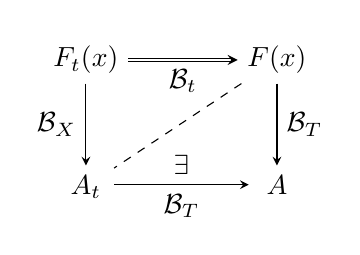
\begin{tikzpicture}
  \matrix (m) [matrix of math nodes,row sep=3em,column sep=4em,minimum width=2em]
  {
     F_t(x) & F(x) \\
     A_t & A \\};
  \path[-stealth]
    (m-1-1) edge node [left] {$\mathcal{B}_X$} (m-2-1)
            edge [double] node [below] {$\mathcal{B}_t$} (m-1-2)
    (m-2-1.east|-m-2-2) edge node [below] {$\mathcal{B}_T$}
            node [above] {$\exists$} (m-2-2)
    (m-1-2) edge node [right] {$\mathcal{B}_T$} (m-2-2)
            edge [dashed,-] (m-2-1);
\end{tikzpicture}
}


{
\tikzstyle{level 1}=[sibling angle=120]
\tikzstyle{level 2}=[sibling angle=60]
\tikzstyle{level 3}=[sibling angle=30]
\tikzstyle{every node}=[fill]
\tikzstyle{edge from parent}=[snake=expanding waves,segment length=1mm,
                              segment angle=10,draw]
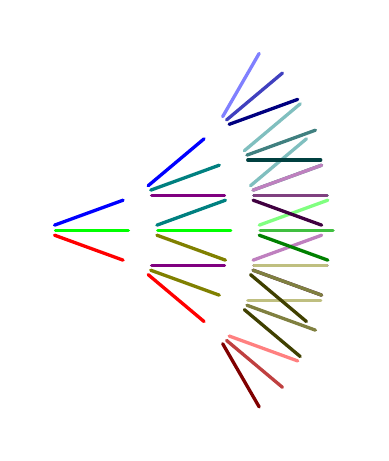
\begin{tikzpicture}[grow cyclic,shape=circle,very thick,level distance=13mm,
                    cap=round]
\node {} child [color=\A] foreach \A in {red,green,blue}
    { node {} child [color=\A!50!\B] foreach \B in {red,green,blue}
        { node {} child [color=\A!50!\B!50!\C] foreach \C in {black,gray,white}
            { node {} }
        }
    };
\end{tikzpicture}
}


A perpendicular bisector of a line segment is a line which is perpendicular
to this line and passes through its midpoint. This drawing shows
perpendicular bisectors of a triangle. They meet in the center of the
circumcircle of the triangle.


{
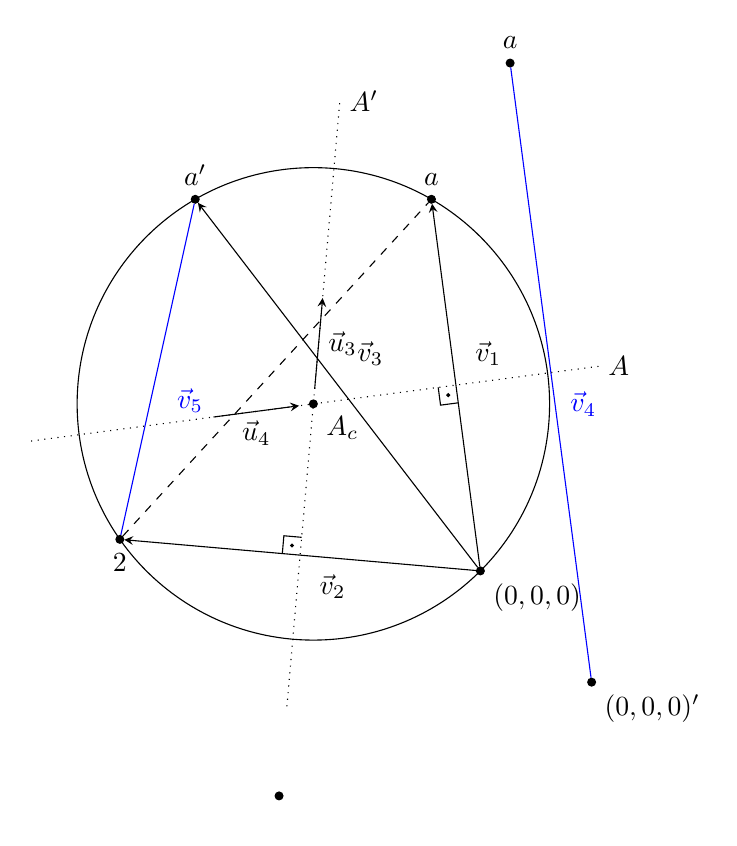
\begin{tikzpicture}
  [
    scale=3,
    >=stealth,
    point/.style = {draw, circle,  fill = black, inner sep = 1pt},
    dot/.style   = {draw, circle,  fill = black, inner sep = .2pt},
  ]

  % the circle
  \def\rad{1}
  \node (origin) at (0,0) [point, label = {below right:$A_c$}]{};
  \draw (origin) circle (\rad);

  % triangle nodes: just points on the circle
  \node (n1) at +(60:\rad) [point, label = above:$a$] {};
  \node (n5) at +(60:1.666*\rad) [point, label = above:$a$] {};
  \node (n4) at +(120:\rad) [point, label = above:$a'$] {};
  \node (n2) at +(-145:\rad) [point, label = below:$2$] {};
  \node (n3) at +(-45:\rad) [point, label = {below right:$(0, 0, 0)$}] {};
  \node (n7) at +(-95:1.666*\rad) [point, label = {below right:}] {};
  \node (n6) at +(-45:1.666*\rad) [point, label = {below right:$(0,  0, 0)'$}] {};

  % triangle edges: connect the vertices, and leave a node at the midpoint
  \draw[->] (n3) -- node (a) [label = {above right:$\vec{v}_1$}] {} (n1);
  \draw[->] (n3) -- node (a') [label = {above right:$\vec{v}_3$}] {} (n4);
  \draw[->] (n3) -- node (b) [label = {below right:$\vec{v}_2$}] {} (n2);
  \draw[blue] (n5) -- node (c) [label = {below right:$\vec{v}_4$}] {} (n6);
  \draw[blue] (n4) -- node (d) [label = {below right:$\vec{v}_5$}] {} (n2);
  \draw[dashed] (n2) -- (n1);

  % Bisectors
  % start at the point lying on the line from (origin) to (a), at
  % twice that distance, and then draw a path going to the point on
  % the line lying on the line from (a) to the (origin), at 3 times
  % that distance.
  \draw[dotted]
    ($ (origin) ! 2 ! (a) $)
    node [right] {$A$}
    -- ($(a) ! 3 ! (origin)$ );

  % similarly for origin and b
  \draw[dotted]
    ($ (origin) ! 2 ! (b) $)
    -- ($(b) ! 3 ! (origin)$ )
    node [right] {$A'$};

  % short vectors
  \draw[->]
    ($ (origin) ! -.7 ! (a) $)
    -- node [below] {$\vec{u}_4$}
    ($ (origin) ! -.1 ! (a) $);
  \draw[->]
    ($ (origin) ! -.1 ! (b) $)
    -- node [right] {$\vec{u}_3$}
    ($ (origin) ! -.7 ! (b) $);

  % Right angle symbols
  \def\ralen{.5ex}  % length of the short segment
  \foreach \inter/\first/\last in {a/n3/origin, b/n2/origin}
    {
      \draw let \p1 = ($(\inter)!\ralen!(\first)$), % point along first path
                \p2 = ($(\inter)!\ralen!(\last)$),  % point along second path
                \p3 = ($(\p1)+(\p2)-(\inter)$)      % corner point
            in
              (\p1) -- (\p3) -- (\p2)               % path
              ($(\inter)!.5!(\p3)$) node [dot] {};  % center dot
    }
\end{tikzpicture}
}


{
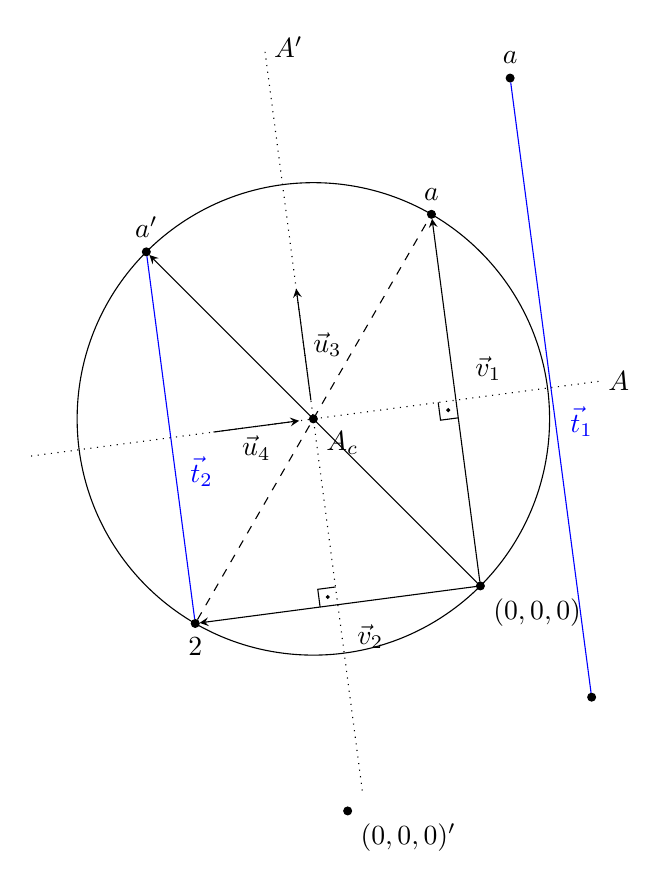
\begin{tikzpicture}
  [
    scale=3,
    >=stealth,
    point/.style = {draw, circle,  fill = black, inner sep = 1pt},
    dot/.style   = {draw, circle,  fill = black, inner sep = .2pt},
  ]

  % the circle
  \def\rad{1}
  \node (origin) at (0,0) [point, label = {below right:$A_c$}]{};
  \draw (origin) circle (\rad);

  % triangle nodes: just points on the circle
  \node (n1) at +(60:\rad) [point, label = above:$a$] {};
  \node (n5) at +(60:1.666*\rad) [point, label = above:$a$] {};
  \node (n4) at +(135:\rad) [point, label = above:$a'$] {};
  \node (n2) at +(-120:\rad) [point, label = below:$2$] {};
  \node (n3) at +(-45:\rad) [point, label = {below right:$(0, 0, 0)$}] {};
  \node (n7) at +(-85:1.666*\rad) [point, label = {below right:$(0, 0, 0)'$}] {};
  \node (n6) at +(-45:1.666*\rad) [point, label = {below right:}] {};

  % triangle edges: connect the vertices, and leave a node at the midpoint
  \draw[->] (n3) -- node (a) [label = {above right:$\vec{v}_1$}] {} (n1);
  \draw[->] (n3) -- node (a') [label = {above right:}] {} (n4);
  \draw[->] (n3) -- node (b) [label = {below right:$\vec{v}_2$}] {} (n2);
  \draw[blue] (n5) -- node (c) [label = {below right:$\vec{t}_1$}] {} (n6);
  \draw[blue] (n4) -- node (d) [label = {below right:$\vec{t}_2$}] {} (n2);
  \draw[dashed] (n2) -- (n1);

  % Bisectors
  % start at the point lying on the line from (origin) to (a), at
  % twice that distance, and then draw a path going to the point on
  % the line lying on the line from (a) to the (origin), at 3 times
  % that distance.
  \draw[dotted]
    ($ (origin) ! 2 ! (a) $)
    node [right] {$A$}
    -- ($(a) ! 3 ! (origin)$ );

  % similarly for origin and b
  \draw[dotted]
    ($ (origin) ! 2 ! (b) $)
    -- ($(b) ! 3 ! (origin)$ )
    node [right] {$A'$};

  % short vectors
  \draw[->]
    ($ (origin) ! -.7 ! (a) $)
    -- node [below] {$\vec{u}_4$}
    ($ (origin) ! -.1 ! (a) $);
  \draw[->]
    ($ (origin) ! -.1 ! (b) $)
    -- node [right] {$\vec{u}_3$}
    ($ (origin) ! -.7 ! (b) $);

  % Right angle symbols
  \def\ralen{.5ex}  % length of the short segment
  \foreach \inter/\first/\last in {a/n3/origin, b/n2/origin}
    {
      \draw let \p1 = ($(\inter)!\ralen!(\first)$), % point along first path
                \p2 = ($(\inter)!\ralen!(\last)$),  % point along second path
                \p3 = ($(\p1)+(\p2)-(\inter)$)      % corner point
            in
              (\p1) -- (\p3) -- (\p2)               % path
              ($(\inter)!.5!(\p3)$) node [dot] {};  % center dot
    }
\end{tikzpicture}
}


{
\tikzset{
    mycomplexfigure/.pic = {
        \draw (-1,-1) rectangle (1,1);
        \draw (0,0) circle (1);
    }
}
\begin{tikzpicture}
\path  (1,2) pic{mycomplexfigure};
\path[blue,rotate=90,transform shape]  (2,1) pic{mycomplexfigure};
\end{tikzpicture}
}



The construction of points on the perpendicular bissector of [AB].
It is achieved in an artisanal way, the purpose being to show how to achieve computations with pgf.
A much simpler construction can certainly be done with other pgf commands but the idea here is to emphasize the analytical process.

{
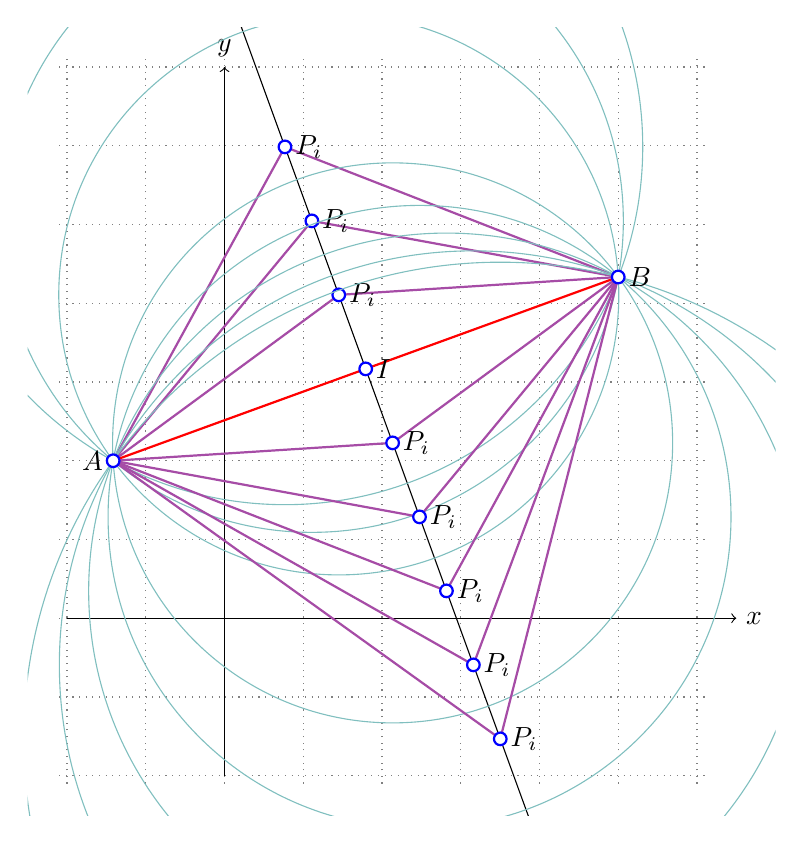
\begin{tikzpicture}[
        scale=1.0,
        MyPoints/.style={draw=blue,fill=white,thick},
        Segments/.style={draw=blue!50!red!70,thick},
        MyCircles/.style={green!50!blue!50,thin}
        ]
    % Warning : all this is an artisanal way of computing points
    % on the perpendicular bissector of [AB]
    % It could very well be achieved with more powerfull tools...
    % (package tkz-2d, for example)
    \clip (-2.5,-2.5) rectangle (7,7.5);
    \draw[color=gray,step=1.0,dotted] (-2.1,-2.1) grid (6.1,7.1);
    \draw[->] (-2,0)--(6.5,0) node[right]{$x$};
    \draw[->] (0,-2)--(0,7) node[above]{$y$};

    % Feel free to change here coordinates of points A and B
    \pgfmathparse{-sqrt(2)}		\let\Xa\pgfmathresult
    \pgfmathparse{2}		\let\Ya\pgfmathresult
    \coordinate (A) at (\Xa,\Ya);
    \pgfmathparse{5}		\let\Xb\pgfmathresult
    \pgfmathparse{13/3}		\let\Yb\pgfmathresult
    \coordinate (B) at (\Xb,\Yb);
    
    % Let I be the midpoint of [AB]
    \pgfmathparse{(\Xb+\Xa)/2} \let\XI\pgfmathresult
    \pgfmathparse{(\Yb+\Ya)/2} \let\YI\pgfmathresult
    \coordinate (I) at (\XI,\YI);	
            
    \draw[red,thick] (A)--(B);
    
    % deltaX and deltaY are coordinates of vector AB
    \pgfmathparse{\Yb-\Ya} \let\deltaY\pgfmathresult
    \pgfmathparse{\Xb-\Xa} \let\deltaX\pgfmathresult
    
    % NormeddeltaX and NormeddeltaY are the normalized values of these coordinates
    \pgfmathparse{sqrt(\deltaX*\deltaX+\deltaY*\deltaY)} \let\r\pgfmathresult
    \pgfmathparse{\deltaX/\r} \let\NormeddeltaX\pgfmathresult
    \pgfmathparse{\deltaY/\r} \let\NormeddeltaY\pgfmathresult

    % R is a point on the perpendicular bissector of [AB],
    % far away from the midpoint...
    \pgfmathparse{\YI-10.0*\NormeddeltaX} \let\YR\pgfmathresult
    \pgfmathparse{\XI+10.0*\NormeddeltaY} \let\XR\pgfmathresult
    
    % S is the image of R by the symmetry of axis AB
    \pgfmathparse{2*\YI-\YR} \let\YS\pgfmathresult
    \pgfmathparse{2*\XI-\XR} \let\XS\pgfmathresult
    \coordinate (R) at (\XR,\YR);
    \coordinate (S) at (\XS,\YS);
    \draw (R)--(S);
    
    \foreach \i in {-3,-2,...,5}{
        \ifthenelse{\equal{\i}{0}}% Do not redraw the segment [AB]
            {}%
            {%
                %\stepcounter{index}
                % P(i) is a variable point on the perpendicular bissector.
                % The distance between P(i) and P(i+1) is equal to 1
                \pgfmathparse{\YI-\i*\NormeddeltaX} \let\YP\pgfmathresult
                \pgfmathparse{\XI+\i*\NormeddeltaY} \let\XP\pgfmathresult
                \coordinate (P) at (\XP,\YP);
                \pgfmathparse{sqrt((\XP-\Xa)*(\XP-\Xa)+(\YP-\Ya)*(\YP-\Ya))}
                \let\radius\pgfmathresult
                            
                \draw[MyCircles] (P) circle ({\radius});
                \draw[Segments] (P)--(A);
                \draw[Segments] (P)--(B);
                %\fill[MyPoints] (P) circle (0.8mm) node[right]{$P_{\theindex}$};
                \fill[MyPoints] (P) circle (0.8mm) node[right]{$P_{i}$};
            }%
        };
        
    \fill[MyPoints] (A) circle (0.8mm) node[left]{$A$};
    \fill[MyPoints] (B) circle (0.8mm) node[right]{$B$};
    \fill[MyPoints] (I) circle (0.8mm) node[right]{$I$};
\end{tikzpicture}
}


Illustration of a `plane partition`.
http://mathworld.wolfram.com/PlanePartition.html

{
\newcounter{x}
\newcounter{y}
\newcounter{z}

% The angles of x,y,z-axes
\newcommand\xaxis{210}
\newcommand\yaxis{-30}
\newcommand\zaxis{90}

% The top side of a cube
\newcommand\topside[3]{
  \fill[fill=yellow, draw=black,shift={(\xaxis:#1)},shift={(\yaxis:#2)},
  shift={(\zaxis:#3)}] (0,0) -- (30:1) -- (0,1) --(150:1)--(0,0);
}

% The left side of a cube
\newcommand\leftside[3]{
  \fill[fill=red, draw=black,shift={(\xaxis:#1)},shift={(\yaxis:#2)},
  shift={(\zaxis:#3)}] (0,0) -- (0,-1) -- (210:1) --(150:1)--(0,0);
}

% The right side of a cube
\newcommand\rightside[3]{
  \fill[fill=blue, draw=black,shift={(\xaxis:#1)},shift={(\yaxis:#2)},
  shift={(\zaxis:#3)}] (0,0) -- (30:1) -- (-30:1) --(0,-1)--(0,0);
}

% The cube 
\newcommand\cube[3]{
  \topside{#1}{#2}{#3} \leftside{#1}{#2}{#3} \rightside{#1}{#2}{#3}
}

% Definition of \planepartition
% To draw the following plane partition, just write \planepartition{ {a, b, c}, {d,e} }.
%  a b c
%  d e
\newcommand\planepartition[1]{
 \setcounter{x}{-1}
  \foreach \a in {#1} {
    \addtocounter{x}{1}
    \setcounter{y}{-1}
    \foreach \b in \a {
      \addtocounter{y}{1}
      \setcounter{z}{-1}
      \foreach \c in {1,...,\b} {
        \addtocounter{z}{1}
        \cube{\value{x}}{\value{y}}{\value{z}}
      }
    }
  }
}


\begin{tikzpicture}
\planepartition{{5,3,2,2},{4,2,2,1},{2,1},{1}}
\end{tikzpicture}
}


The width and height of the triangle are put into constants, so we can change
them later if we need to. Loading them once and computing everything else on
the fly, it makes it easier to change things around later

We label our coordinates so that the name matches the label which gets printed,
otherwise we might get horribly confused.

Two of the rectangles (the ones matching the horizontal and vertical edges)
are easy to draw. The square corresponding to the hypotenuse is a bit
more difficult, but we can use a little plane geometry. We can find another
edge of the square by rotating the original triangle through 90 degrees,
and then translating appropriately. We can use the same method to find the
two extra coordinates of the hypotenuse square in TikZ.

{
\newcommand{\pythagwidth}{3cm}
\newcommand{\pythagheight}{2cm}
\begin{tikzpicture}
  \coordinate [label={below right:$A$}] (A) at (0, 0);
  \coordinate [label={above right:$B$}] (B) at (0, \pythagheight);
  \coordinate [label={below left:$C$}] (C) at (-\pythagwidth, 0);

  \coordinate (D1) at (-\pythagheight, \pythagheight + \pythagwidth);
  \coordinate (D2) at (-\pythagheight - \pythagwidth, \pythagwidth);

  \draw [very thick] (A) -- (C) -- (B) -- (A);

  \newcommand{\ranglesize}{0.3cm}
  \draw (A) -- ++ (0, \ranglesize) -- ++ (-\ranglesize, 0) -- ++ (0, -\ranglesize);

  \draw [dashed] (A) -- node [below] {$b$} ++ (-\pythagwidth, 0)
            -- node [right] {$b$} ++ (0, -\pythagwidth)
            -- node [above] {$b$} ++ (\pythagwidth, 0)
            -- node [left]  {$b$} ++ (0, \pythagwidth);

  \draw [dashed] (A) -- node [right] {$c$} ++ (0, \pythagheight)
            -- node [below] {$c$} ++ (\pythagheight, 0)
            -- node [left]  {$c$} ++ (0, -\pythagheight)
            -- node [above] {$c$} ++ (-\pythagheight, 0);

  \draw [dashed] (C) -- node [above left]  {$a$} (B)
                     -- node [below left]  {$a$} (D1)
                     -- node [below right] {$a$} (D2)
                     -- node [above right] {$a$} (C);
\end{tikzpicture}
}


{
\def\r{4}
\def\n{8} \def\myangles{{25,50,85,125,160,220,250,280,340}}
%This vector contains the angles determining the position of the points.
%-----------------------------------------------------------
% Variables and counters used to generate the 4-combinations
\newcounter{np} \pgfmathsetcounter{np}{\n+1}
\newcounter{na} \newcounter{nb} \newcounter{nc}
\newcounter{ia} 
\pgfmathsetcounter{na}{\n-1}    % saves some computations later
\pgfmathsetcounter{nb}{\n-2}    % ""
\pgfmathsetcounter{nc}{\n-3}    %   ""
\newcounter{q} \setcounter{q}{0}    % if flag q=1 then exit the whiledo loop
\newcounter{e} \setcounter{e}{0}    % e counts the combinations!
\newcounter{a} \setcounter{a}{0}    % element of the 4-combination
\newcounter{b} \setcounter{b}{1}    % ""
\newcounter{c} \setcounter{c}{2}    % ""
\newcounter{d} \setcounter{d}{2}    % ""
%Watch out! The initial value {0,1,2,2} is not a 4-combination
%-----------------------------------------------------------

Consider $n$ randomly placed points on a circle.

\begin{enumerate}
    \item The complete graph on the $n$ points has $\begin{pmatrix}n\\2\end{pmatrix}$ edges.
    \item Each pair of edges yields an intersection point and there are (at most) $\begin{pmatrix}n\\4\end{pmatrix}$ such points.
\end{enumerate}

\begin{tikzpicture}
    % Draw the complete graph
    \fill[fill=blue!10!green!10!,draw=blue,dotted,thick] (0,0) circle (\r);
    \pgfmathparse{\n-1} \let\nn\pgfmathresult 
    \foreach \i in {0,...,\nn}{
        \pgfmathparse{\i+1} \let\ii\pgfmathresult
        \pgfmathparse{\myangles[\i]} \let\t\pgfmathresult
        \foreach \j in {\ii,...,\n}
            \pgfmathparse{\myangles[\j]} \let\u\pgfmathresult
            \draw[blue,very thick] ({\r*cos(\t)},{\r*sin(\t)})--({\r*cos(\u)},{\r*sin(\u)});
        }
    \foreach \i in {0,...,\n}{
        \pgfmathparse{\myangles[\i]}    \let\t\pgfmathresult
        \pgfmathsetcounter{ia}{\i+1}
        \fill[draw=blue,fill=blue!20!,thick]
                ({\r*cos(\t)},{\r*sin(\t)})circle (2.5mm) node{$\mathbf{\theia}$};
        }
        % Points and segments are now drawn
        %
    \whiledo{\theq=0}{ % this loop generates the 4-combinations
        \stepcounter{e}
        \ifthenelse{\thee=1000}{\setcounter{q}{1}}{}% just to be sure to get out of the loop some day...
        \ifthenelse{\thed=\n}
            {\ifthenelse{\thec=\thena}
                {\ifthenelse{\theb=\thenb}
                    {\ifthenelse{\thea=\thenc}
                        {\setcounter{q}{1}}
                        {   \stepcounter{a}
                            \pgfmathsetcounter{b}{\thea+1}
                            \pgfmathsetcounter{c}{\thea+2}
                            \pgfmathsetcounter{d}{\thea+3}                  
                        }
                    }
                    {   \stepcounter{b}
                        \pgfmathsetcounter{c}{\theb+1}
                        \pgfmathsetcounter{d}{\theb+2}                      
                    }
                }
                {   \stepcounter{c}
                    \pgfmathsetcounter{d}{\thec+1}
                }
            }
            {\stepcounter{d}}
        \ifthenelse{\theq=0}{
            % Construction of the intersection points of the segments
            \pgfmathparse{\r*cos(\myangles[\thea])} \let\xa\pgfmathresult
            \pgfmathparse{\r*sin(\myangles[\thea])} \let\ya\pgfmathresult
            \pgfmathparse{\r*cos(\myangles[\theb])} \let\xb\pgfmathresult
            \pgfmathparse{\r*sin(\myangles[\theb])} \let\yb\pgfmathresult
            \pgfmathparse{\r*cos(\myangles[\thec])} \let\xc\pgfmathresult
            \pgfmathparse{\r*sin(\myangles[\thec])} \let\yc\pgfmathresult
            \pgfmathparse{\r*cos(\myangles[\thed])} \let\xd\pgfmathresult
            \pgfmathparse{\r*sin(\myangles[\thed])} \let\yd\pgfmathresult
            %               
            \coordinate  (A) at (\xa,\ya);
            \coordinate  (B) at (\xb,\yb);
            \coordinate  (C) at (\xc,\yc);
            \coordinate  (D) at (\xd,\yd);
            % Name the coordinates, but do not draw anything!               
            \path[name path=sega] (A) -- (C);
            \path[name path=segb] (B) -- (D);
            \path [name intersections={of=sega and segb}];
            \coordinate (X) at (intersection-1);
            \fill[fill=green!50!,draw=blue] (X) circle (0.8mm);             
            %-----------------------------------------------------
            }{}
    }% End of the whiledo loop
\end{tikzpicture}
}


{
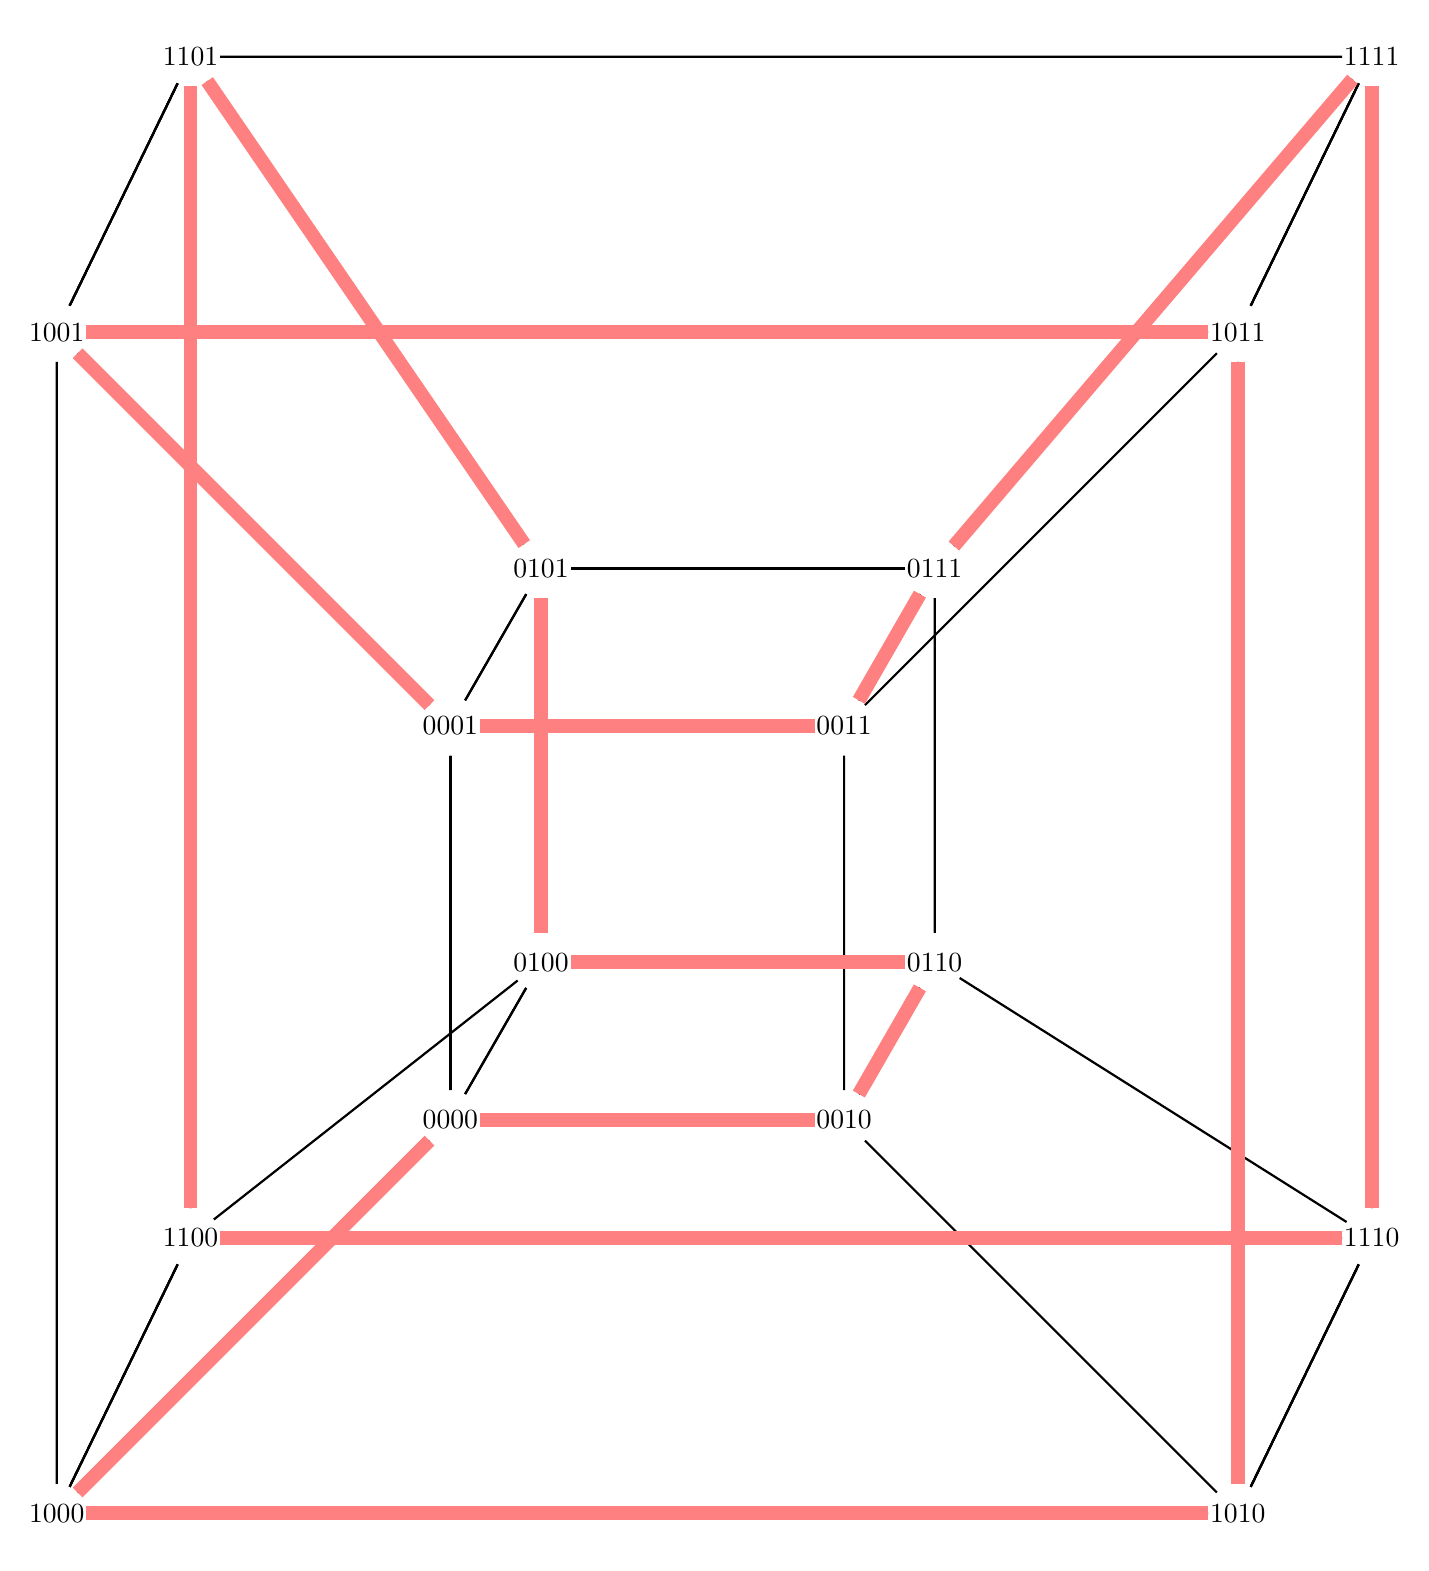
\begin{tikzpicture}[scale=5]
	 \tikzstyle{vertex}=[circle,minimum size=20pt,inner sep=0pt]
	 \tikzstyle{selected vertex} = [vertex, fill=red!24]
	 \tikzstyle{selected edge} = [draw,line width=5pt,-,red!50]
	 \tikzstyle{edge} = [draw,thick,-,black]
	 \node[vertex] (v0) at (0,0) {$0000$};
	 \node[vertex] (v1) at (0,1) {$0001$};
	 \node[vertex] (v2) at (1,0) {$0010$};
	 \node[vertex] (v3) at (1,1) {$0011$};
	 \node[vertex] (v4) at (0.23, 0.4) {$0100$};
	 \node[vertex] (v5) at (0.23,1.4) {$0101$};
	 \node[vertex] (v6) at (1.23,0.4) {$0110$};
	 \node[vertex] (v7) at (1.23,1.4) {$0111$};
	 \node[vertex] (v8) at (-1,-1) {$1000$};
	 \node[vertex] (v9) at (-1,2) {$1001$};
	 \node[vertex] (v13) at (-0.66,2.7) {$1101$};
	 \node[vertex] (v12) at (-0.66,-0.3) {$1100$};
	 \node[vertex] (v10) at (2,-1) {$1010$};
	 \node[vertex] (v14) at (2.34,-0.3) {$1110$};
	 \node[vertex] (v11) at (2,2) {$1011$};
	 \node[vertex] (v15) at (2.34,2.7) {$1111$};
	 \draw[edge] (v0) -- (v1) -- (v3) -- (v2) -- (v0);
	 \draw[edge] (v0) -- (v4) -- (v5) -- (v1) -- (v0);
	 \draw[edge] (v2) -- (v6) -- (v7) -- (v3) -- (v2);
	 \draw[edge] (v4) -- (v6) -- (v7) -- (v5) -- (v4);
	 \draw[edge] (v8) -- (v9) -- (v13) -- (v12) -- (v8);
	 \draw[edge] (v0) -- (v4) -- (v12) -- (v8) -- (v0);
	 \draw[edge] (v1) -- (v9) -- (v13) -- (v5) -- (v1);
	 \draw[edge] (v2) -- (v10) -- (v14) -- (v6) -- (v2);
	 \draw[edge] (v8) -- (v10) -- (v14) -- (v12) -- (v8);
	 \draw[edge] (v3) -- (v11) -- (v15) -- (v7) -- (v3);
	 \draw[edge] (v10) -- (v11) -- (v15) -- (v14) -- (v10);
	 \draw[edge] (v9) -- (v11) -- (v15) -- (v13) -- (v9);
	 \draw[selected edge] (v0) -- (v2);
	 \draw[selected edge] (v2) -- (v6);
	 \draw[selected edge] (v6) -- (v4);
	 \draw[selected edge] (v4) -- (v5);
	 \draw[selected edge] (v5) -- (v13);
	 \draw[selected edge] (v13) -- (v12);
	 \draw[selected edge] (v12) -- (v14);
	 \draw[selected edge] (v14) -- (v15);
	 \draw[selected edge] (v15) -- (v7);
	 \draw[selected edge] (v7) -- (v3);
	 \draw[selected edge] (v3) -- (v1);
	 \draw[selected edge] (v1) -- (v9);
	 \draw[selected edge] (v9) -- (v11);
	 \draw[selected edge] (v11) -- (v10);
	 \draw[selected edge] (v10) -- (v8);
	 \draw[selected edge] (v8) -- (v0);
 \end{tikzpicture}
}


{
\tikzstyle{every node}=[circle, draw, fill=black!50,
                        inner sep=0pt, minimum width=4pt]
%  Tutte's 8-cage
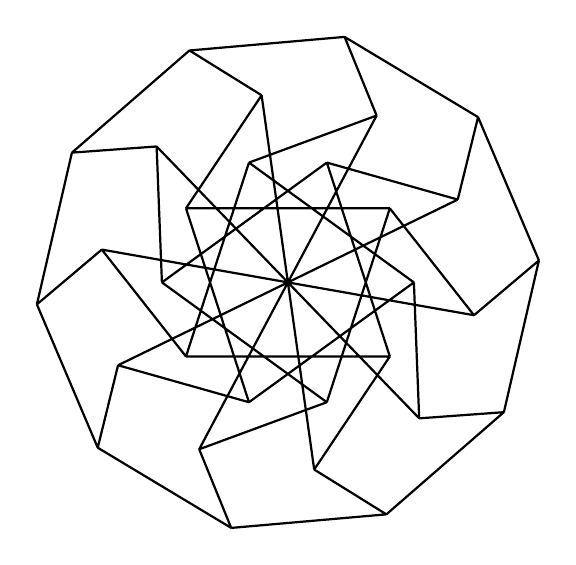
\begin{tikzpicture}[thick,scale=0.8]
    % The following path utilizes several useful tricks and features:
    % 1) The foreach statement is put inside a path, so all the edges
    %    will in fact be a the same path.
    % 2) The node construct is used to draw the nodes. Nodes are special
    %    in the way that they are drawn *after* the path is drawn. This
    %    is very useful in this case because the nodes will be drawn on
    %    top of the path and therefore hide all edge joins.
    % 3) Simple arithmetics can be used when specifying coordinates.
    \draw \foreach \x in {0,36,...,324}
    {
        (\x:2) node {}  -- (\x+108:2)
        (\x-10:3) node {} -- (\x+5:4)
        (\x-10:3) -- (\x+36:2)
        (\x-10:3) --(\x+170:3)
        (\x+5:4) node {} -- (\x+41:4)
    };
\end{tikzpicture}\quad
%
%
% The largest 3-regular graph of diameter 3
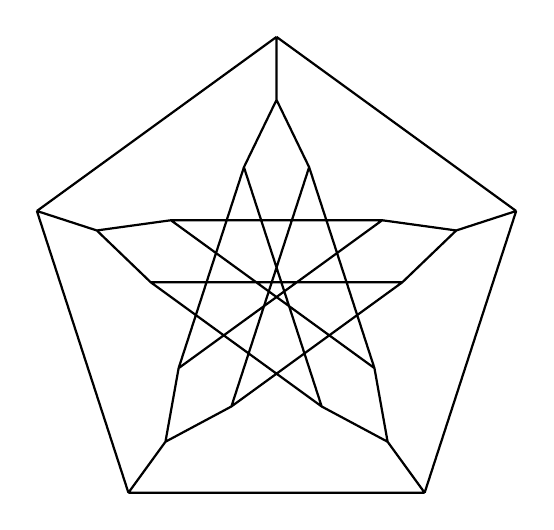
\begin{tikzpicture}[thick,scale=0.8]%
    \draw \foreach \x in {18,90,...,306} {
        (\x:4) node{} -- (\x+72:4)
        (\x:4) -- (\x:3) node{}
        (\x:3) -- (\x+15:2) node{}
        (\x:3) -- (\x-15:2) node{}
        (\x+15:2) -- (\x+144-15:2)
        (\x-15:2) -- (\x+144+15:2)
};
\end{tikzpicture}
}






\end{document}https://www.overleaf.com/project/5d85406fddb1a00001ce4700
